\documentclass[twoside]{book}

% Packages required by doxygen
\usepackage{fixltx2e}
\usepackage{calc}
\usepackage{doxygen}
\usepackage[export]{adjustbox} % also loads graphicx
\usepackage{graphicx}
\usepackage[utf8]{inputenc}
\usepackage{makeidx}
\usepackage{multicol}
\usepackage{multirow}
\PassOptionsToPackage{warn}{textcomp}
\usepackage{textcomp}
\usepackage[nointegrals]{wasysym}
\usepackage[table]{xcolor}

% Font selection
\usepackage[T1]{fontenc}
\usepackage[scaled=.90]{helvet}
\usepackage{courier}
\usepackage{amssymb}
\usepackage{sectsty}
\renewcommand{\familydefault}{\sfdefault}
\allsectionsfont{%
  \fontseries{bc}\selectfont%
  \color{darkgray}%
}
\renewcommand{\DoxyLabelFont}{%
  \fontseries{bc}\selectfont%
  \color{darkgray}%
}
\newcommand{\+}{\discretionary{\mbox{\scriptsize$\hookleftarrow$}}{}{}}

% Page & text layout
\usepackage{geometry}
\geometry{%
  a4paper,%
  top=2.5cm,%
  bottom=2.5cm,%
  left=2.5cm,%
  right=2.5cm%
}
\tolerance=750
\hfuzz=15pt
\hbadness=750
\setlength{\emergencystretch}{15pt}
\setlength{\parindent}{0cm}
\setlength{\parskip}{3ex plus 2ex minus 2ex}
\makeatletter
\renewcommand{\paragraph}{%
  \@startsection{paragraph}{4}{0ex}{-1.0ex}{1.0ex}{%
    \normalfont\normalsize\bfseries\SS@parafont%
  }%
}
\renewcommand{\subparagraph}{%
  \@startsection{subparagraph}{5}{0ex}{-1.0ex}{1.0ex}{%
    \normalfont\normalsize\bfseries\SS@subparafont%
  }%
}
\makeatother

% Headers & footers
\usepackage{fancyhdr}
\pagestyle{fancyplain}
\fancyhead[LE]{\fancyplain{}{\bfseries\thepage}}
\fancyhead[CE]{\fancyplain{}{}}
\fancyhead[RE]{\fancyplain{}{\bfseries\leftmark}}
\fancyhead[LO]{\fancyplain{}{\bfseries\rightmark}}
\fancyhead[CO]{\fancyplain{}{}}
\fancyhead[RO]{\fancyplain{}{\bfseries\thepage}}
\fancyfoot[LE]{\fancyplain{}{}}
\fancyfoot[CE]{\fancyplain{}{}}
\fancyfoot[RE]{\fancyplain{}{\bfseries\scriptsize Generated by Doxygen }}
\fancyfoot[LO]{\fancyplain{}{\bfseries\scriptsize Generated by Doxygen }}
\fancyfoot[CO]{\fancyplain{}{}}
\fancyfoot[RO]{\fancyplain{}{}}
\renewcommand{\footrulewidth}{0.4pt}
\renewcommand{\chaptermark}[1]{%
  \markboth{#1}{}%
}
\renewcommand{\sectionmark}[1]{%
  \markright{\thesection\ #1}%
}

% Indices & bibliography
\usepackage{natbib}
\usepackage[titles]{tocloft}
\setcounter{tocdepth}{3}
\setcounter{secnumdepth}{5}
\makeindex

% Hyperlinks (required, but should be loaded last)
\usepackage{ifpdf}
\ifpdf
  \usepackage[pdftex,pagebackref=true]{hyperref}
\else
  \usepackage[ps2pdf,pagebackref=true]{hyperref}
\fi
\hypersetup{%
  colorlinks=true,%
  linkcolor=blue,%
  citecolor=blue,%
  unicode%
}

% Custom commands
\newcommand{\clearemptydoublepage}{%
  \newpage{\pagestyle{empty}\cleardoublepage}%
}

\usepackage{caption}
\captionsetup{labelsep=space,justification=centering,font={bf},singlelinecheck=off,skip=4pt,position=top}

%===== C O N T E N T S =====

\begin{document}

% Titlepage & ToC
\hypersetup{pageanchor=false,
             bookmarksnumbered=true,
             pdfencoding=unicode
            }
\pagenumbering{alph}
\begin{titlepage}
\vspace*{7cm}
\begin{center}%
{\Large Vinhos v0.1 }\\
\vspace*{1cm}
{\large Generated by Doxygen 1.8.13}\\
\end{center}
\end{titlepage}
\clearemptydoublepage
\pagenumbering{roman}
\tableofcontents
\clearemptydoublepage
\pagenumbering{arabic}
\hypersetup{pageanchor=true}

%--- Begin generated contents ---
\chapter{Hierarchical Index}
\section{Class Hierarchy}
This inheritance list is sorted roughly, but not completely, alphabetically\+:\begin{DoxyCompactList}
\item \contentsline{section}{Interface\+Handler}{\pageref{class_interface_handler}}{}
\item Q\+Main\+Window\begin{DoxyCompactList}
\item \contentsline{section}{Vinhos}{\pageref{class_vinhos}}{}
\end{DoxyCompactList}
\item \contentsline{section}{qt\+\_\+meta\+\_\+stringdata\+\_\+\+Vinhos\+\_\+t}{\pageref{structqt__meta__stringdata___vinhos__t}}{}
\item \contentsline{section}{Ui\+\_\+\+Vinhos\+Class}{\pageref{class_ui___vinhos_class}}{}
\begin{DoxyCompactList}
\item \contentsline{section}{Ui\+:\+:Vinhos\+Class}{\pageref{class_ui_1_1_vinhos_class}}{}
\end{DoxyCompactList}
\end{DoxyCompactList}

\chapter{Class Index}
\section{Class List}
Here are the classes, structs, unions and interfaces with brief descriptions\+:\begin{DoxyCompactList}
\item\contentsline{section}{\hyperlink{class_interface_handler}{Interface\+Handler} }{\pageref{class_interface_handler}}{}
\item\contentsline{section}{\hyperlink{structqt__meta__stringdata___vinhos__t}{qt\+\_\+meta\+\_\+stringdata\+\_\+\+Vinhos\+\_\+t} }{\pageref{structqt__meta__stringdata___vinhos__t}}{}
\item\contentsline{section}{\hyperlink{class_ui___vinhos_class}{Ui\+\_\+\+Vinhos\+Class} }{\pageref{class_ui___vinhos_class}}{}
\item\contentsline{section}{\hyperlink{class_vinhos}{Vinhos} }{\pageref{class_vinhos}}{}
\item\contentsline{section}{\hyperlink{class_ui_1_1_vinhos_class}{Ui\+::\+Vinhos\+Class} }{\pageref{class_ui_1_1_vinhos_class}}{}
\end{DoxyCompactList}

\chapter{Class Documentation}
\hypertarget{class_interface_handler}{}\section{Interface\+Handler Class Reference}
\label{class_interface_handler}\index{Interface\+Handler@{Interface\+Handler}}


The documentation for this class was generated from the following files\+:\begin{DoxyCompactItemize}
\item 
Vinhos/Interface\+Handler.\+h\item 
Vinhos/Interface\+Handler.\+cpp\end{DoxyCompactItemize}

\hypertarget{structqt__meta__stringdata___vinhos__t}{}\section{qt\+\_\+meta\+\_\+stringdata\+\_\+\+Vinhos\+\_\+t Struct Reference}
\label{structqt__meta__stringdata___vinhos__t}\index{qt\+\_\+meta\+\_\+stringdata\+\_\+\+Vinhos\+\_\+t@{qt\+\_\+meta\+\_\+stringdata\+\_\+\+Vinhos\+\_\+t}}
\subsection*{Public Attributes}
\begin{DoxyCompactItemize}
\item 
\mbox{\Hypertarget{structqt__meta__stringdata___vinhos__t_a6d76a5b9032e67aefa965cbe8bddea8a}\label{structqt__meta__stringdata___vinhos__t_a6d76a5b9032e67aefa965cbe8bddea8a}} 
Q\+Byte\+Array\+Data {\bfseries data} \mbox{[}1\mbox{]}
\item 
\mbox{\Hypertarget{structqt__meta__stringdata___vinhos__t_a90b0f4f3d276be386b01fa64609a409e}\label{structqt__meta__stringdata___vinhos__t_a90b0f4f3d276be386b01fa64609a409e}} 
char {\bfseries stringdata0} \mbox{[}7\mbox{]}
\end{DoxyCompactItemize}


The documentation for this struct was generated from the following file\+:\begin{DoxyCompactItemize}
\item 
Vinhos/\+Generated\+Files/\+Debug/moc\+\_\+\+Vinhos.\+cpp\end{DoxyCompactItemize}

\hypertarget{class_ui___vinhos_class}{}\section{Ui\+\_\+\+Vinhos\+Class Class Reference}
\label{class_ui___vinhos_class}\index{Ui\+\_\+\+Vinhos\+Class@{Ui\+\_\+\+Vinhos\+Class}}
Inheritance diagram for Ui\+\_\+\+Vinhos\+Class\+:\begin{figure}[H]
\begin{center}
\leavevmode
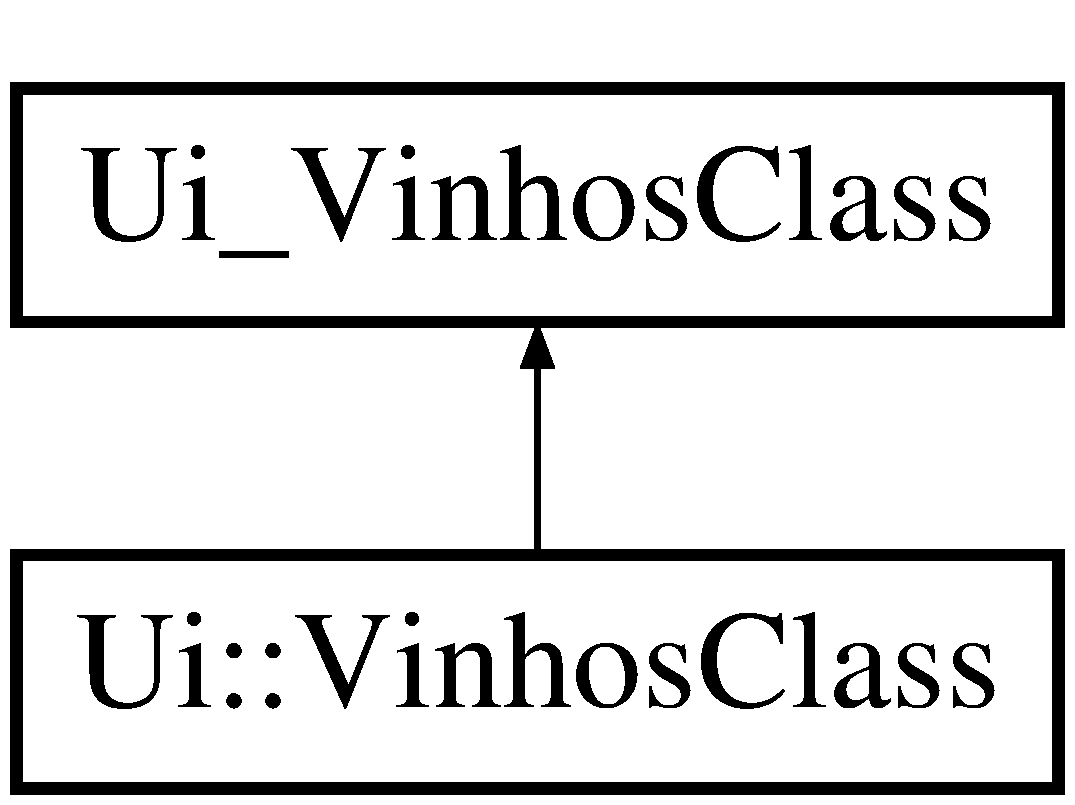
\includegraphics[height=2.000000cm]{class_ui___vinhos_class}
\end{center}
\end{figure}
\subsection*{Public Member Functions}
\begin{DoxyCompactItemize}
\item 
\mbox{\Hypertarget{class_ui___vinhos_class_ab30c3a295a5cdddc4e9e5fe022cad3f1}\label{class_ui___vinhos_class_ab30c3a295a5cdddc4e9e5fe022cad3f1}} 
void {\bfseries setup\+Ui} (Q\+Main\+Window $\ast$Vinhos\+Class)
\item 
\mbox{\Hypertarget{class_ui___vinhos_class_a7d4ff86c37ed4aac53052fc8d3032c0f}\label{class_ui___vinhos_class_a7d4ff86c37ed4aac53052fc8d3032c0f}} 
void {\bfseries retranslate\+Ui} (Q\+Main\+Window $\ast$Vinhos\+Class)
\end{DoxyCompactItemize}
\subsection*{Public Attributes}
\begin{DoxyCompactItemize}
\item 
\mbox{\Hypertarget{class_ui___vinhos_class_a095c73e52be913a9815ac8f903403f08}\label{class_ui___vinhos_class_a095c73e52be913a9815ac8f903403f08}} 
Q\+Menu\+Bar $\ast$ {\bfseries menu\+Bar}
\item 
\mbox{\Hypertarget{class_ui___vinhos_class_af36d65eb16343fffa006f1b5e83a06e9}\label{class_ui___vinhos_class_af36d65eb16343fffa006f1b5e83a06e9}} 
Q\+Tool\+Bar $\ast$ {\bfseries main\+Tool\+Bar}
\item 
\mbox{\Hypertarget{class_ui___vinhos_class_a304fba6c5f17885055d58f21be247429}\label{class_ui___vinhos_class_a304fba6c5f17885055d58f21be247429}} 
Q\+Widget $\ast$ {\bfseries central\+Widget}
\item 
\mbox{\Hypertarget{class_ui___vinhos_class_aa9bde5c3cc3de9a74a1fc3d59abd4414}\label{class_ui___vinhos_class_aa9bde5c3cc3de9a74a1fc3d59abd4414}} 
Q\+Status\+Bar $\ast$ {\bfseries status\+Bar}
\end{DoxyCompactItemize}


The documentation for this class was generated from the following file\+:\begin{DoxyCompactItemize}
\item 
Vinhos/\+Generated\+Files/ui\+\_\+\+Vinhos.\+h\end{DoxyCompactItemize}

\hypertarget{class_vinhos}{}\section{Vinhos Class Reference}
\label{class_vinhos}\index{Vinhos@{Vinhos}}
Inheritance diagram for Vinhos\+:\begin{figure}[H]
\begin{center}
\leavevmode
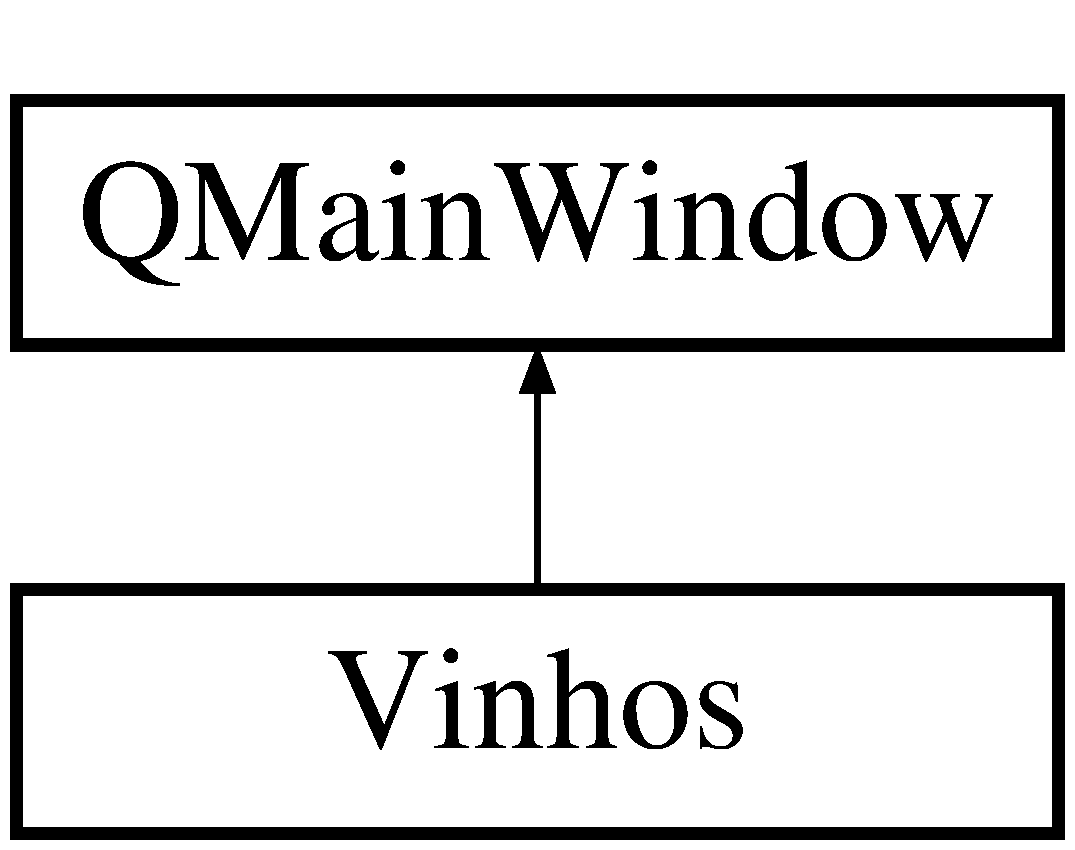
\includegraphics[height=2.000000cm]{class_vinhos}
\end{center}
\end{figure}
\subsection*{Public Member Functions}
\begin{DoxyCompactItemize}
\item 
\mbox{\Hypertarget{class_vinhos_ad12ae5857e2aac003b7f95e89fba5250}\label{class_vinhos_ad12ae5857e2aac003b7f95e89fba5250}} 
{\bfseries Vinhos} (Q\+Widget $\ast$parent=Q\+\_\+\+N\+U\+L\+L\+P\+TR)
\end{DoxyCompactItemize}


The documentation for this class was generated from the following files\+:\begin{DoxyCompactItemize}
\item 
Vinhos/Vinhos.\+h\item 
Vinhos/Vinhos.\+cpp\end{DoxyCompactItemize}

\hypertarget{class_ui_1_1_vinhos_class}{}\section{Ui\+:\+:Vinhos\+Class Class Reference}
\label{class_ui_1_1_vinhos_class}\index{Ui\+::\+Vinhos\+Class@{Ui\+::\+Vinhos\+Class}}
Inheritance diagram for Ui\+:\+:Vinhos\+Class\+:\begin{figure}[H]
\begin{center}
\leavevmode
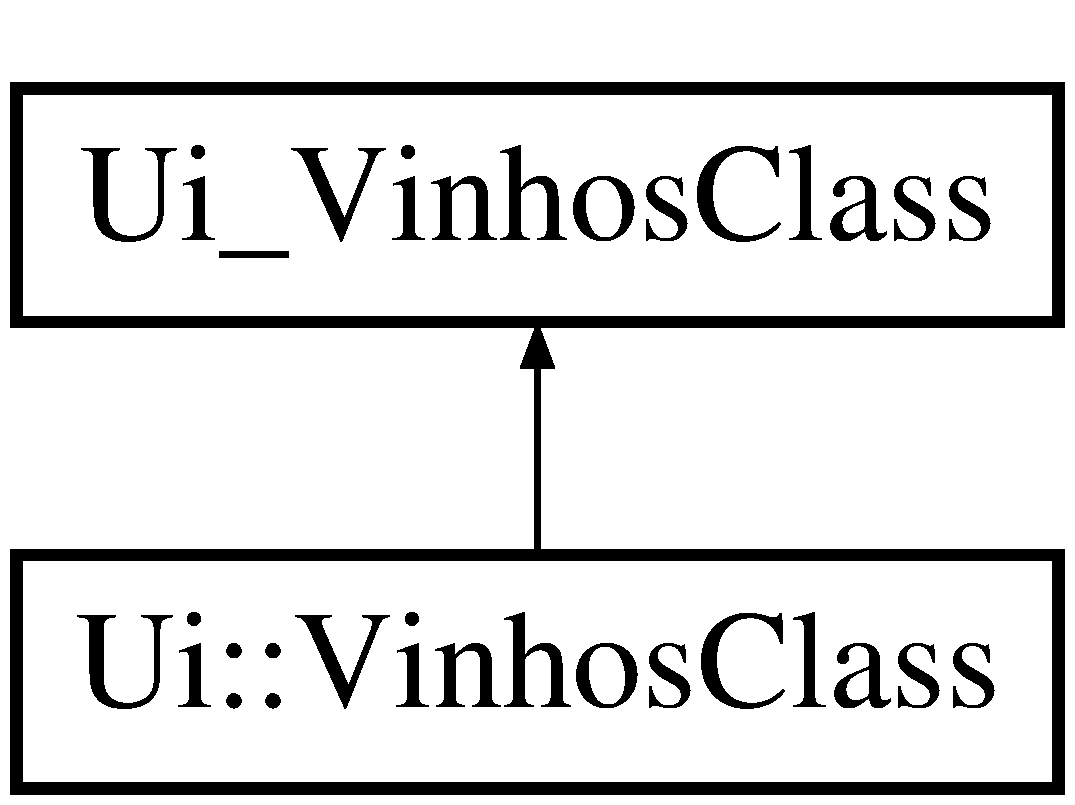
\includegraphics[height=2.000000cm]{class_ui_1_1_vinhos_class}
\end{center}
\end{figure}
\subsection*{Additional Inherited Members}


The documentation for this class was generated from the following file\+:\begin{DoxyCompactItemize}
\item 
Vinhos/\+Generated\+Files/ui\+\_\+\+Vinhos.\+h\end{DoxyCompactItemize}

%--- End generated contents ---

% Index
\backmatter
\newpage
\phantomsection
\clearemptydoublepage
\addcontentsline{toc}{chapter}{Index}
\printindex

\end{document}
